%%%%%%%%%%%%%%%%%%%%%%%%%%%%%%%%%%%%%%%%%%%%%%%%%%%%%%%%%%%%%%%%%%%%%%%%%%%%%%%%
%2345678901234567890123456789012345678901234567890123456789012345678901234567890
%        1         2         3         4         5         6         7         8

\documentclass[10pt, conference, compsocconf]{IEEEtran}
  % Comment this line out
                                                          % if you need a4paper
%\documentclass[a4paper, 10pt, conference]{IEEEtran}      % Use this line for a4
                                                          % paper

% See the \addtolength command later in the file to balance the column lengths
% on the last page of the document



% The following packages can be found on http:\\www.ctan.org
\usepackage{graphics} % for pdf, bitmapped graphics files
\usepackage{epsfig} % for postscript graphics files
\usepackage{subfigure} % for subfigures
\usepackage{caption}
%\usepackage{mathptmx} % assumes new font selection scheme installed
%\usepackage{times} % assumes new font selection scheme installed
%\usepackage{amsmath} % assumes amsmath package installed
%\usepackage{amssymb}  % assumes amsmath package installd

% for algorithm
\usepackage[noend]{algpseudocode}
\usepackage{algorithm}

\usepackage{mycommands,amsmath,amssymb,amsthm,hyperref,cite}

\title{\LARGE \bf
A fast and accurate denoising technique for high-resolution image streams using data depth-based robust kernel PCA
}

\DeclareMathOperator*{\argmin}{arg\,min}
\DeclareMathOperator*{\argmax}{arg\,max}

\begin{document}

%\DeclareMathOperator*{\diag}{diag}
%\DeclareMathOperator*{\Tr}{Tr}


%\newtheorem{Theorem}{Theorem}[section]
%\newtheorem{Lemma}[Theorem]{Lemma}
%\newtheorem{Corollary}[Theorem]{Corollary}
%\theoremstyle{definition} \newtheorem{Definition}[Theorem]{Definition}
\newtheorem{proposition}{Proposition}
\newtheorem{theorem}{Theorem}
\theoremstyle{definition} \newtheorem{definition}{Definition}

\author{\IEEEauthorblockN{Subhabrata Majumdar, Abhirup Mallik}
\IEEEauthorblockA{School of Statistics\\
University of Minnesota - Twin Cities\\
Minneapolis, MN, USA\\
Email: majum010@umn.edu; malli066@umn.edu}}

\maketitle
\thispagestyle{empty}
\pagestyle{empty}

%%%%%%%%%%%%%%%%%%%%%%%%%%%%%%%%%%%%%%%%%%%%%%%%%%%%%%%%%%%%%%%%%%%%%%%%%%%%%%%%
\begin{abstract}

Classical kernel principal component analysis (PCA) has been shown to be quite sensitive to the presence of outliers, so many robust versions of kernel PCA exists in the literature. However, they suffer from lack of scalability with increasing amount of data and less accuracy compared to the classical version. Here we propose to use multivariate ranks obtained using data depth calculated in kernel spaces to get a robust version of kernel PCA applicable in big data scenarios, for example, denoising of large images. Given the kernel matrix, the extra calculation required here on top of classical kernel PCA does not grow with number of features, hence being more scalable. We provide theoretical properties related to the method, as well as demonstrate its effectiveness through simulations and a real data application. We also propose a scheme to outline how to use our method to check a continuous stream of images for noise, and denoise them if necessary.
\end{abstract}

\begin{IEEEkeywords}
Big data; image denoising; data depth; kernel PCA; robust PCA
\end{IEEEkeywords}

%%%%%%%%%%%%%%%%%%%%%%%%%%%%%%%%%%%%%%%%%%%%%%%%%%%%%%%%%%%%%%%%%%%%%%%%%%%%%%%%
\section{INTRODUCTION}

We propose a fast, robust and efficient method of doing principal component analysis (PCA) in kernel spaces. This method extends upon the idea of doing PCA on multivariate rank vectors based on data depth in place of original data \cite{Majumdar15}. The time required for this modification does not increase with dimension of the feature space from which data are drawn, thus making it scalable for data with very high number of features. For this reason, the method will be specifically useful in denoising streams of high-resolution images in real time, which is a relevant problem in medical\cite{Ouahabi13} and Geographic Information System (GIS) imaging\cite{YeMohamadian}. It is also possible to adapt our method to existing algorithms of kernel PCA that are fast as well as have less time and memory complexity, like the Kernel Hebbian Algorithm\cite{KimFranzSchol05} or Incremental Kernel PCA\cite{OzawaTakeuchiAbe10}, to make them robust.

Image denoising techniques can be divided into two general classes. The first class of methods divide an image into blocks and use local blurring and often parallel computing using CPU or GPU \cite{nvidia}. These methods require increasing amount of computation time for high-resolution images. On the other hand, the second class of methods adapt robust linear PCA methods in kernel settings. These estimators typically have high breakdown points but suffer from poor efficiency compared to classical PCA\cite{taskinen12, hubert05}. The above difficulties make both types of methods difficult to implement in real-time scenarios involving high-resolution images. Compared to them, our simple modification using data depth is capable of accurately reconstructing original images from projections of noisy images on kernel spaces, as well as robust and fast estimation of the underlying kernel subspace from batch-wise processing of incoming data.

Data depth provides a scalar measure for the `center outward ordering' of a multivariate point with respect to some data cloud\cite{zuo00}. Most depth functions available in the literature generate convex contours irrespective to the shape of the data cloud, and are unsuitable for distributions that have more than one mode or non-convex support \cite{Paindaveine13}, which are often encountered in real life. Moreover, calculation of depth functions are often computationally expensive. These two reasons make depth-based methods unsuitable for application in big data scenario. Here we bypass both difficulties by using kernelized spatial depth \cite{Chen09}, that respects the local geometry around a data point and given the sample kernel matrix, calculates its depth in time that increases quadratically with sample size, irrespective of the number of features.

This article is organized as follows. Section II reviews the theoretical groundwork required for our analysis by introducing key concepts related to PCA, kernel methods and data depth. Based on these concepts, in section III we obtain theoretical results related to depth-based kernel PCA, explicitly deriving the modified kernel matrix and score vectors corresponding to our method. Sections IV and V demonstrate the performance of our method through simulations and a real data example, respectively. In section VI we introduce a quality index measuring the amount of noise in an incoming image, and based on that provide an algorithm for batch-wise processing and optional denoising of a stream of high-resolution images using our method. We end this paper by providing the summary of our work and motivating further areas of application in section VII. The appendix supplies proofs of the results we state in the main content.

\section{Preliminaries}\label{section:sec2}

\subsection{Kernel Principal Component Analysis}

Given a random variable $\bfX$ with mean $\bf0$ taking values in $\mathbb{R}^p$, principal components are defined as columns of the orthogonal matrix $\bfW = (\bfw_1, ... ,\bfw_p)^T$ so that

\begin{eqnarray}
\bfw_1 &=& \argmin_{\| \bfw \| = 1} \bfw^T \bfX^T\bfX \bfw \\
\bfw_k &=& \argmin_{\| \bfw \| = 1} \bfw^T \hat \bfX^T_k \hat \bfX_k \bfw
\end{eqnarray}
$$ \mbox{ with } \hat \bfX_k = \bfX - \sum_{s=1}^{k-1} \bfw_s \bfw_s^T \bfX \mbox{ for } k = 2,...,p $$

The vectors $\bfw_k$ turn out to be eigenvectors of the covariance matrix of $\bfX$ ordered according to the corresponding decreasing eigenvalues. This change of coordinates works well in dimension reduction when the data lies in a linear subspace of dimension lower than feature space, but not so much for data with inherent nonlinearity among variables. In this scenario, we use kernel PCA \cite{Scholkopf99} instead. We map the data to a new (potentially higher dimensional) feature space through a nonlinear transformation $\phi: \mathbb{R}^p \mapsto \mathbb R^D$, and perform standard PCA on the transformed variables.

To bypass explicit computation of the function $\phi$, we apply the `kernel trick'. Given $n$ random draws $\bfX_1,...,\bfX_n$, the $k^\text{th}$ eigen                                                                                                                                                                              vector ($1\leq k \leq P$) in the transformed space can be written as a linear combination of the transformed samples: $\bfv_k = \sum_{i=1}^n a_{ki} \phi (\bfx_i)$, and given centered transformations, i.e. $\sum_{i=1}^n \phi(\bfx_i) = \bf0$, we obtain the vector of coefficients $\bfa_k = (a_{k1},...,a_{kn})^T$ as solution of the following equation:

\begin{equation}
K \bfa_k = n \lambda_k \bfa_k
\end{equation}
using the kernel function induced by the transformation: $k( \bfa, \bfb) = \phi(\bfa)^T \phi(\bfb)$, for $\bfa, \bfb \in \mathbb R^p$, so that $K_{n \times n}$ has $(i,j)^\text{th}$ element $k(\bfx_i, \bfx_j)$ and $\lambda_k$ is the $k^\text{th}$ eigenvalue of the covariance matrix of transformed observations, i.e. $E( \phi(\bfX) \phi(\bfX)^T )$.

Following this, we can obtain the $k^\text{th}$ principal component score for $\bfx \in \mathbb R$:
\begin{equation}
s_k (\bfx) = \bfv_k^T \phi (\bfx) = \sum_{i=1}^n a_{ki} k( \bfx, \bfx_i)
\end{equation}

Some frquently used kernels in this context are:

\begin{itemize}
\item \textit{Gaussian kernel}: $k(\bfa, \bfb) = \exp ( - \| \bfa - \bfb \|^2 / 2 \sigma); \sigma>0 $
\item \textit{Polynomial kernel}: $k(\bfa, \bfb) = (\bfa^T \bfb)^d; d>0$
\item \textit{Sigmoid kernel}: $k(\bfa, \bfb) = \tanh (\eta \bfa^T \bfb + \nu)$
\end{itemize}
Note that setting $d = 1$ in a polynomial kernel results in the usual inner product, or the so-called uniform kernel.

%and the projection of any $\phi(\bfx) \in \mathcal F$ can be written as
%
%\begin{equation}
%\hat\bfv_k = \sum_{i=1}^n a_{ki} \phi(\bfx_i)^T \phi(\bfx) = \sum_{i=1}^n a_{ki} k( \bfx, \bfx_i )
%\end{equation}

\subsection{Depth functions, and kernel depth}
Given a data cloud or a probability distribution, a depth function is any real-valued function that measures the outlyingness of a point in feature space with respect to the data or its underlying distribution. In order to formalize the notion of depth, we consider as data depth any scalar-valued function $D(\bfx, F_\bfX)$ (where $\bfx \in \mathbb R^p$, and the random variable $\bfX$ has distribution $F$) that satisfies the following properties \cite{Liu90}:

\begin{itemize}
\item \textit{P1. Affine invariance}: $D(A\bfx + \bfb, F_{A\bfX + \bfb}) = D(\bfx, F_\bfX)$ for any $p \times p$ non-singular matrix $A$ and $p \times 1$ vector $\bfb$;

\item \textit{P2. Maximality at center}: When $F_\bfX$ has center of symmetry $\bftheta$, $D(\bftheta, F_\bfX) = \sup_{\bfx \in \mathbb R^p} D(\bfx, F_\bfX)$. Here the symmetry can be central, angular or halfspace symmetry;

\item \textit{P3. Monotonicity relative to deepest point}: For any $p \times 1$ vector $\bfx$ and $\alpha \in [0,1]$, $D(\bfx, F_\bfX) \leq D(\bftheta + a(\bfx - \bftheta))$;

\item \textit{P4. Vanishing at infinity}: As $\| \bfx \| \rightarrow \infty$, $D(\bfx, F_\bfX) \rightarrow 0$.
\end{itemize}

Among depth functions, spatial depth is especially attractive because of its computationally frugal nature (time complexity $O(n^2)$). The spatial depth of a point $\bfx \in \mathbb{R}^p$ with respect to a distribution $F$ is defined as:

\begin{equation}
D(\bfx, F) = 1 - \left\| \int \bfS(\bfy - \bfx) dF(\bfy) \right\|
\end{equation}
where $\bfS(\bfx) = \bfx / \| \bfx \|$ is the spatial sign functional. For $n$ random draws $\mathcal{X} = \{ \bfx_1, ... , \bfx_n \}$ we estimate the population spatial depth by its sample version, in which the integral is replaced by average over all sample points. Its kernelized version \cite{Chen09} defined below allows us fast computation of depths \textit{and} depth contours that respect the shape of the data cloud.

\begin{definition}[Chen \textit{et al}\cite{Chen09}]
Consider any kernel function $k$. Then in the above setup, the \textit{sample kernelized spatial depth} for any $\bfx \in \mathbb{R}^p$ is defined as:

\begin{equation}
\begin{split}
D_k(\bfx, \mathcal{X}) = 1 - \frac{1}{| \mathcal{X} \cup \bfx | - 1} \times \qquad\qquad\\
\left( \sum_{\bfy, \bfz \in \mathcal{X}} \frac{k(\bfx, \bfx) + k(\bfy, \bfz) - k(\bfx, \bfy) - k(\bfx, \bfz)}{\delta_k(\bfx, \bfy) \delta_k(\bfx, \bfz)}\right)^{1/2}
\end{split}
\end{equation}
where $\delta_k (\bfx, \bfy) = \sqrt{k(\bfx, \bfx) + k(\bfy, \bfy) - 2k(\bfx, \bfy)}$.
\end{definition}

Subsequently, we can easily infer the following:

\begin{proposition}\label{prop:prop1}
For any transformation $\phi$ as considered above, and $k$ being the kernel induced by the transformation, consider random samples $\mathcal X$ and an arbitrary point $\bfx \in \mathbb R^p$. Then we have

\begin{equation}
D_k(\bfx, \mathcal X) = D( \phi(\bfx), \phi(\mathcal X))
\end{equation}
when $D$ is spatial depth and $D_k$ is kernelized spatial depth.
\end{proposition}

\section{Depth-based PCA and its kernelized version}\label{section:sec3}

When the underlying data distribution is elliptic, data depth can be used to estimate population eigenvectors in a robust and fairly efficient fashion \cite{Majumdar15}. For this, suppose the distribution is centered at $\bfmu \in \mathbb R^p$ and any depth function $D$. Then we define the multivariate rank vector $\tilde \bfx = \tilde D(\bfx, F_\bfX)(\bfx - \bfmu)/\| \bfx - \bfmu \|$, where $\tilde D(\bfx, F_\bfX) = \exp(-D(\bfx, F_\bfX))$ is the outlyingness or \textit{htped function} corresponding to $D$. After this we simply do PCA on these vectors in place of original data vectors.

Here we assume that the transformed random variable $\phi(\bfX)$ follows an elliptical distribution, centered at $\bftheta = \phi(\bfmu)$. In this setup multivariate ranks are defined in the new feature space:

\begin{eqnarray}
\phi_D(\bfx) &=& \tilde D( \phi(\bfx), \phi(\mathcal X)). \bfS( \phi(\bfx) - \phi(\bfmu))\nonumber\\
&=& \tilde D_k( \bfx, \mathcal X) \frac{\phi(\bfx) - \phi(\bfmu)}{\sqrt{k(\bfx - \bfmu, \bfx - \bfmu)}}
\end{eqnarray}

When the center is unknown, following the case of spherical kernel PCA \cite{DeBruyne10} i.e. kernel PCA on spatial sign vectors in the feature space, we estimate it by the spatial median, i.e. solution $\hat \bftheta$ to the following equation:

\begin{equation}
\sum_{i=1}^n \frac{\phi(\bfx_i) - \hat \bftheta}{\| \phi(\bfx_i) - \hat \bftheta \|} = {\bf 0}
\end{equation}
This is calculated using a simple iterative algorithm and the kernel function as a linear combination of the samples: $\hat\bftheta = \sum_{i=1}^n \gamma_i \phi(\bfx_i)$. Finally, we obtain the kernel matrix $K_D$ induced by the transformation $\phi_D$:

\begin{theorem}\label{thm:thm1}
Given that the center of the transformed distribution is estimated by the spatial median as above, the matrix $K_D$ with $k_D( \bfx_i, \bfx_j) := \phi_D(\bfx_i)^T \phi_D(\bfx_j)$ in its $(i,j)^\text{th}$ position has the form:

\begin{equation}\label{eqn:thm1Eqn}
K_D = \Lambda_D K_\Gamma \Lambda_D; \quad K_\Gamma = K + \Gamma^T K \Gamma - \Gamma^T K - K \Gamma
\end{equation}
where $\Gamma$ is a $n \times n$ matrix with $\bfgamma = (\gamma_1,...,\gamma_n)^T$ as each of its columns, and $\Lambda_D$ is a diagonal matrix with diagonal elements $\lambda_{D,ii} := \tilde D_k(\bfx_i, \mathcal X)/ \sqrt{K_{\Gamma,ii}}$.
\end{theorem}

We now perform PCA on the multivariate ranks in the transformed space, i.e. $\{ \phi_D(\bfx_1), ... , \phi_D(\bfx_n) \}$. Given that the estimate of the $k^\text{th}$ eigenvector is $\bfv^D_k = \sum_{i=1}^n a^D_{ki} \phi_D(\bfx_i)$, the score due to $k^\text{th}$ principal component is:

\begin{eqnarray}
s_k^D(\bfx) &=& \sum_{i=1}^n a^D_{ki} \phi_D(\bfx_i)^T \left[ \phi(\bfx) - \hat\bftheta \right]\notag\\
&=& \sum_{i=1}^n a^D_{ki} \lambda_{D,ii} \times \notag\\
&& \hspace{-.5cm} \left[ k(\bfx, \bfx_i) + \bfgamma^T K \bfgamma  - k(\bfx, \hat\bftheta) - k(\bfx_i, \hat\bftheta) \right]
\end{eqnarray}
using the expansion of $\hat\bftheta$.

%% Include algorithm
%% explain choice of kernel tuning param.. gaussian.. single sigma, and diagonal Sigma and non-diagonal Sigma
\section{Simulations}\label{section:sec4}
\subsection{Effect of the number of features}
We first set up our simulation study following the framework used by Mika \textit{et al}\cite{Mikaetal99}. We generated a data set of eleven Gaussians in $\mathbb{R}^{10}$ with means chosen randomly in $[-1,1]^{10}$, and variance $\sigma^2=1$ in each component. We took training and test sets of size 100 and 33 for each of distributions, and carried out three different kinds of Kernel PCA: classical (kCPCA), spherical (kSPCA) and depth-based (kDPCA). We used the principal components from the training data to recover the points in the test data and calculated the mean squared errors (MSE) in the recovered points and the original points using different number of components. The result is shown in Figure \ref{fig:sim1}. We can see as more components are being used, the MSE in general decreases as expected. However kDPCA performs relatively better than all other methods when we are using fewer components.

\subsection{Effect of number of outliers}
We now recreate the simulation setup used by Yang \textit{et al}\cite{Yangetal14}. The purpose of this experiment is to explore the nature of robustness between several version of robust PCA. The data set used is a two dimensional synthetic dataset $\mathcal{X}:\{x_i,y_i\}_{i=1}^n$ (we used $n=101$) where $x_i$ were generated from $U[0,1]$. We obtained the responses as $y_i = 0.5\sin(2\pi x_i)+0.5+0.1r_i$, with $r_i \sim N(0,1)$ being independently generated standard gaussian noise. Outliers were generated from $N(5,1)$ distribution. The ratio of the data to outliers were varied from 20\% to 50\%. To measure robustness, we compared first eigenvector estimates on the original data using kCPCA and corrupted data using kSPCA and kDPCA using absolute cosine distance, which is defined below:

\begin{align*}
\text{distance}(\bfgamma_1, \bfgamma_2) =& \cos^{-1} | \bfgamma_1^T \bfgamma_2 |
\end{align*}
We compare how the number of outliers affect the principal components based on this distance in figure \ref{fig:sim2}. It seems that as number of outliers increase, the distance between eigenvectors increases at first, then they decrease. Here in this set up after using 18 outliers, we see an decrease. However in all cases, depth-based PCA had lesser distance to the PC from kernel PCA.

\section{Application: fast and accurate image denoising}\label{section:sec5}

We use the extended Yale Face Database B (\cite{GeBeKr01,KcLee05}) in this  example to demonstrate efficacy of our method. We compare its outputs with the same from classical kernel PCA and spherical kernel PCA. The score vectors returned by any kernel PCA method reside in the transformed space, so to apply kernel PCA in image processing, it is imperative to get back pre-images in the original space corresponding to these score vectors. We use the fast and stable method proposed by Kwok and Tsang that approximates pre-images by the multivariate basis spanned by a fixed number ($k$) of nearest sample points in the feature space\cite{KwokTsang03}. For our purpose we fix $k=5$. We use gaussian kernel as our chosen kernel function, and obtain the optimal bandwidth $\hat\sigma$ as:

\begin{equation}
\frac{1}{2\hat\sigma} = \frac{1}{n(n-1)} \sum_{i=1}^n \sum_{j=1}^n \| \bfx_i - \bfx_j \|^2
\end{equation}

Here we take 20 grayscale images each for three persons (samples yaleB01, yaleB02 and yaleB28, to be exact) under the same order of lighting conditions. From here on we shall refer to them as person 1, 2 and 3, respectively. We choose the persons so that their facial features are very different. We read in the images in their original resolution ($192 \times 168$). After this we select 25\% pixels at random from 7$^\text{th}$ images for each person and turn their pixel values to 0 or 1 with probability 0.5. Known as \textit{speckle noise}, this type of noise is common in several imaging techniques, and causes degradation of image quality as well as bad performance of image classification algorithms\cite{Qiuetal04}. After addition of noise, we take each of the 60 images as a vector of length $192\times 168 = 32256$, extract kernel principal components from the $60 \times 32256$ dataset by the three methods under consideration and feed the 3 corrupted images into the models in order to denoise them.

\subsection{Image reconstruction}

Panel (a) of figure \ref{fig:yale1} shows the three original images and their corrupted versions, and panels (b), (c) and (d) show their denoised versions. The five rows correspond to number of kernel principal components used in reconstruction (2, 4, 6, 8 or 10), while the three columns show reconstructions obtained by  kCPCA, kSPCA and kDPCA, respectively. In general, kDPCA performs best among the methods for all three images. The method of reconstruction we consider here approximates pre-image of some projection by a basis spanned by only 5 among 60 sample points. An inaccurate estimation of underlying kernel principal components due to one or more corrupted sample point(s) can result in images that belong to different persons being selected among nearest neighbors of the projection of a corrupted image. Here we see that kSPCA suffers from this in all three images. For person 1, reconstructions using 2 and 4 spherical kernel PCs obtain an image belonging to person 2, while all reconstructions of persons 2 and 3 using this method gives back images of person 1 and 2 instead. This reiterates on the fact that non-kernel spherical PCA is considerably less efficient than non-kernel classical PCA when the underlying data distribution is multivariate normal (\cite{magyar14, Majumdar15}).

The kCPCA denoisings are comparatively better, except for images 4 and 5 for person 3. Denoised images of persons 1 and 2 turn out to be darker than corresponding original images. kDPCA does not suffer from any of these disadvantages, and accurately denoises all three corrupted images.

\subsection{Signal-to-Noise Ratio comparison}

We also calculate the Signal-to-Noise Ratios (SNR) of these images and compare them to those of corresponding noisy images. Here we consider a noisy image as signal, and given the original image, pixel-wise difference of the noisy and original images is taken as noise. SNR is simply defined as ratio of the mean pixel value in signal image and standard deviation of noise. Higher SNR of a denoised image compared to noisy image corresponds to a better denoising.

In table \ref{table:SNRtable} we list the calculated SNRs. Among the 15 denoisings we consider here, kDPCA has highest SNR among 3 methods for 8 of them. Almost all kDPCA denoisings (except 2 PC denoising for person 2) have higher SNRs than original noisy images. Some more interesting observations are:

\begin{itemize}
\item For person 1, kDPCA consistently provides very high SNR.
\item For person 2, using 10 PCs and kDPCA gives very good denoising, which is also evident from the corresponding image in figure \ref{fig:yale1}.
\item For person 3, using a higher number of PCs deteriorates the performance of kCPCA, but kDPCA still gives higher SNR than noisy image.
\end{itemize}

Note that a high SNR does not necessarily translate to an accurate reconstructed image in our scenario. Images of person 2 obtained by kCPCA are darker than the original image in general, but still have highest SNR when 4, 6 or 8 PCs are used. For the same person, when using 2 PCs kSPCA gives highest SNR, although in the plot we see that it returns person 1's image instead.

\section{Real-time denoising of high-resolution image sequences}

Since kDPCA does not suffer from the dreaded `curse of dimensionality', its main advantage lies in application on data with very high amount of features, which in our context can be pixel data from high-resolution images. Based on the above outputs, we propose below a scheme of denoising an incoming stream of images using kDPCA. For an image with high amount of noise, we can expect a large difference of pixel values between this image and its denoised version using kDPCA. Keeping this mind, we define the following to quantify the difference:

\begin{definition}
Given two images, say $I_0$ and $I_1$, the \textit{Mean Standardized difference} (MSD) between the images is defined as

\begin{equation}
\text{MSD}(I_0, I_1) = \frac{| \text{mean} (v(I_0) - v(I_1)) |}{\text{sd}(v(I_0) - v(I_1))}
\end{equation}
where for some image $I$, $v(I)$ is a vector containing all pixel values in $I$.
\end{definition}

To do real-time image denoising, we first use MSD values for a small set of initial training images and use a fixed quantile of these values (for example, 95\% or 99\%) as threshold. After that we consider a smaller block of incoming images, denoise and calculate their MSD, and compare them with the threshold obtained from the training sample. For images whose MSD values exceed the threshold we store the denoised image instead of the original image. Finally we update the training set by including `good' test images, i.e. test images that have below-threshold MSD, and discarding equal number of images from the start of the old training set. After this we take in another block of incoming image and repeat the process. A formal sketch of the above scheme is given in algorithm \ref{alg:algorecon}.

\begin{algorithm}
\caption{Algorithm for fast real-time image denoising using kDPCA}
\label{alg:algorecon}
\begin{algorithmic}[1]
\Procedure{KdpcaDenoise} {stream of images $\{I_1,I_2,...\}$}

\State Fix integers $N,n \in \mathbb{N}, N>n$; cutoff probability $c$.
\State Initialize training set of images $T = \{ I_1, ..., I_N\}$.
\State Set test set starting position $p=0$.

\State \emph{train}:
\State Use $T$ to build a kDPCA model $\mathcal{M}_T$.
\State Denoise images in $T$ using $\mathcal{M}_T$ and get $T' = \{ I_1', ..., I_N'\}$.
\State Calculate their MSDs
$$m_i := \text{MSD}(I_i, I_i')$$
for $i = 1,2,...,N$.
\State Set $C = c^\text{th}$ quantile of $m_1,...,m_N$.

\State \emph{test}:
\State Read in test set of images $S = \{I_{N+p+1}, ... ,I_{N+p+n}\}$.
\State Use $\mathcal{M}_T$ to denoise images in $S$ and get $S' = \{I_{N+p+1}', ... ,I_{N+p+n}'\}$.
\State Get their MSDs: $m_{N+p+1},...,m_{N+p+n}$.
\For {$i\textbf{ in } 1:n$}
\If {$m_{N+p+i} > C$}
\State Set $I_{N+p+i} \leftarrow I_{N+p+i}'$
\EndIf
\EndFor

\State \emph{update}:
\State Set $j=1$.
\For {$i\textbf{ in } 1:n$}
\If {$m_{N+p+i} < C$}
\State Set $T \leftarrow T - \{I_j\} \cup \{I_{N+p+i}\}$
\State Set $j \leftarrow j+1$
\EndIf
\EndFor
\State Set $p \leftarrow p+n$, \textbf{goto} \emph{train}

\EndProcedure
\end{algorithmic}
\end{algorithm}

We choose not to include the denoised images in training samples because their MSD values are extreme compared to those of other, `good' images in training set. To build a kDPCA model, the only extra calculation compared to an (often inefficient) kSPCA model we need to do is due to calculating kernelized depth values of samples. In an updated train sample one can either calculate depths of all $N$ points, which has time complexity $O(N^2)$; or only calculate depths for new training samples and recycle depths for other points. In this case the extra computation time required will be only $O(n_k^2)$, where $n_k$ is the number of new training samples introduced.

\section{Conclusion}\label{section:end}

In the above sections we outline a robust version of kernel PCA that is fast, provides accurate reconstructions, and most importantly can be scaled to denoise data streams with non-regular shape features that have large amount of features as well as samples. As extension, we think that since the quantity MSD adapts to the constantly updated training data, it can be used as a tool for anomaly or changepoint detection in similar type of data. Also the estimation and reconstruction in kDPCA using gaussian kernels can potentially be improved by using diagonal or positive definite matrices as the tuning covariance matrix instead of a single scalar quantity $\sigma$.

% start with the scheme. mention extensions: anomaly detection from image streams, cite Beigi, Chang, Ebadollahi, Verma

%\addtolength{\textheight}{-12cm}   % This command serves to balance the column lengths
                                  % on the last page of the document manually. It shortens
                                  % the textheight of the last page by a suitable amount.
                                  % This command does not take effect until the next page
                                  % so it should come on the page before the last. Make
                                  % sure that you do not shorten the textheight too much.

%%%%%%%%%%%%%%%%%%%%%%%%%%%%%%%%%%%%%%%%%%%%%%%%%%%%%%%%%%%%%%%%%%%%%%%%%%%%%%%%

\section*{Appendix}

\begin{proof}[Proof of proposition \ref{prop:prop1}]
For the transformed data in $\mathbb{R}^D$, the sample spatial depth can be written as \cite{Chen09}:

$$ D( \phi(\bfX), \phi(\mathcal{X})) = 1 - \frac{1}{| \mathcal{X} \cup \bfx | - 1} \left\| \sum_{\bfy \in \mathcal{X}} \bfS (\phi(\bfy) - \phi(\bfx)) \right\| $$
Next we break down the square of the norm above and rewrite using only kernel inner products, making it free of $\phi$ hence estimable from the given data:

\begin{eqnarray*}
&&\left\| \sum_{\bfy \in \mathcal{X}} \bfS (\phi(\bfy) - \phi(\bfx)) \right\|^2\\
&=& \sum_{\bfy, \bfz \in \mathcal{X}} \left( \bfS (\phi(\bfx) - \phi(\bfy)) \right)^T \bfS (\phi(\bfx) - \phi(\bfz)) \\
&=& \sum_{\bfy, \bfz \in \mathcal{X}} \frac{ (\phi(\bfx) - \phi(\bfy))^T(\phi(\bfx) - \phi(\bfz))}{\| \phi(\bfx) - \phi(\bfy) \| \| \phi(\bfx) - \phi(\bfz) \|} \\
&=& \sum_{\bfy, \bfz \in \mathcal{X}} \frac{ \phi(\bfx)^T\phi(\bfx) + \phi(\bfy)^T\phi(\bfz) - \phi(\bfx)^T\phi(\bfy) - \phi(\bfx)^T\phi(\bfz)}{\| \phi(\bfx) - \phi(\bfy) \| \| \phi(\bfx) - \phi(\bfz) \|} \\
&=& \sum_{\bfy, \bfz \in \mathcal{X}} \frac{k(\bfx, \bfx) + k(\bfy, \bfz) - k(\bfx, \bfy) - k(\bfx, \bfz)}{\delta_k(\bfx, \bfy) \delta_k(\bfx, \bfz)}
\end{eqnarray*}
and the result follows from the definition of $D_k(\bfx, \mathcal{X})$.
\end{proof}

\begin{proof}[Proof of Theorem \ref{thm:thm1}]
$K_\Gamma$ is essentially the kernel matrix corresponding to all observations centered at the spatial median. To see that, we look at the $(i,j)^\text{th}$ element of the kernel matrix for centered observations:

\begin{eqnarray*}
&& k(\bfx_i-\bfmu, \bfx_j-\bfmu)\\
&=& k(\bfx_i, \bfx_j) - k(\bfx_i, \bfmu) - k(\bfx_j, \bfmu) + k(\bfmu, \bfmu)\\
&=& k(\bfx_i, \bfx_j) + \sum_{k=1}^n \sum_{l=1}^n \gamma_k \gamma_l k(\bfx_k, \bfx_l) \\
&& - \sum_{k=1}^n \gamma_k k(\bfx_i, \bfx_k) - \sum_{k=1}^n \gamma_k k(\bfx_j, \bfx_k) \\
\end{eqnarray*}
The first term is $(i,j)^\text{th}$ element of $K$, second term is constant for all $(i,j)$, and the third and fourth terms are cross-products of $\bfgamma$ with $i^\text{th}$ and $j^\text{th}$ rows (or columns) of $K$, respectively. Accumulating all terms and writing them in matrix notation we get the expansion for $K_\Gamma$ in \ref{eqn:thm1Eqn}.

Now we only need to expand $k_D(\bfx_i, \bfx_j)$:
\begin{eqnarray*}
&&\phi_D(\bfx_i)^T \phi_D(\bfx_j)\\
&=& \tilde D_k (\bfx_i, \mathcal X) \tilde D_k (\bfx_j, \mathcal X) \times\\
&& \frac{k(\bfx_i-\bfmu, \bfx_j-\bfmu)}{\sqrt{k(\bfx_i-\bfmu, \bfx_i-\bfmu)}\sqrt{k(\bfx_j-\bfmu, \bfx_j-\bfmu)}}\\
&=& \frac{\tilde D_k (\bfx_i, \mathcal X)}{\sqrt{K_{\Gamma,ii}}} K_{\Gamma,ij} \frac{\tilde D_k (\bfx_j, \mathcal X)}{\sqrt{K_{\Gamma,jj}}}
\end{eqnarray*}
to conclude the needed.
\end{proof}

\section*{Acknowledgment}

This research is partially supported by the United States National Science Foundation grant IIS--1029711. We thank our doctoral adviser Prof. Snigdhansu Chatterjee for his valuable guidance.

%%%%%%%%%%%%%%%%%%%%%%%%%%%%%%%%%%%%%%%%%%%%%%%%%%%%%%%%%%%%%%%%%%%%%%%%%%%%%%%%

%References are important to the reader; therefore, each citation must be complete and correct. If at all possible, references should be commonly available publications.

\bibliography{IEEEtranBST/IEEEabrv,kdpca}
\bibliographystyle{IEEEtranBST/IEEEtran}

%%%%%%%%%%%%%%%%%%%%%%%%%%%%%%%%%%%%%%%%%%%%%%%%%%%%%%%%%%%%%%%%%%%%%%%%%%%%%%%%%

\begin{table*}[b]
\begin{center}
    \begin{tabular}{c|c|ccc}
    \hline
   Image           & No. of     & \multicolumn{3}{c}{SNR}\\\cline{3-5}
                   & kernel PCs & kCPCA & kSPCA & kDPCA \\ \hline
    ~              & 2          & 1.26  & 1.48  & \textbf{4.99}  \\
    Corrupted      & 4          & 1.16  & 1.56  & \textbf{5.81}  \\
    Image 1,       & 6          & 1.42  & 3.03  & \textbf{5.80}  \\
    SNR = 1.94     & 8          & 1.55  & \textbf{6.33}  & 6.30  \\
    ~              & 10         & 1.55  & 3.30  & \textbf{8.05}  \\ \hline
    ~              & 2          & 1.67  & \textbf{2.13}  & 1.46  \\
    Corrupted      & 4          & \textbf{1.97}  & 1.01  & 1.60  \\
    Image 2,       & 6          & \textbf{1.91}  & 1.05  & 1.56  \\
    SNR = 1.51     & 8          & \textbf{1.97}  & 1.48  & 1.60  \\
    ~              & 10         & 1.65  & 1.47  & \textbf{5.72}  \\ \hline
    ~              & 2          & 1.65  & 0.90  & \textbf{1.73}  \\
    Corrupted      & 4          & \textbf{2.31}  & 1.11  & 2.13  \\
    Image 2,       & 6          & \textbf{2.31}  & 1.04  & 1.82  \\
    SNR = 1.44     & 8          & 0.85  & 1.46  & \textbf{2.01}  \\
    ~              & 10         & 0.80  & 0.95  & \textbf{1.63}  \\ \hline
    \end{tabular}
\end{center}
\caption{Signal-to-noise ratios of reconstructions by 3 methods of kernel PCA}
\label{table:SNRtable}
\end{table*}

%%%%%%%%%%%%%%%%%%%%%%%%%%%%%%%%%%%%%%%%%%%%%%%%%%%%%%%%%%%%%%%%%%%%%%%%%%%%%%%%%
\clearpage

\begin{figure*}[htp]
\centering
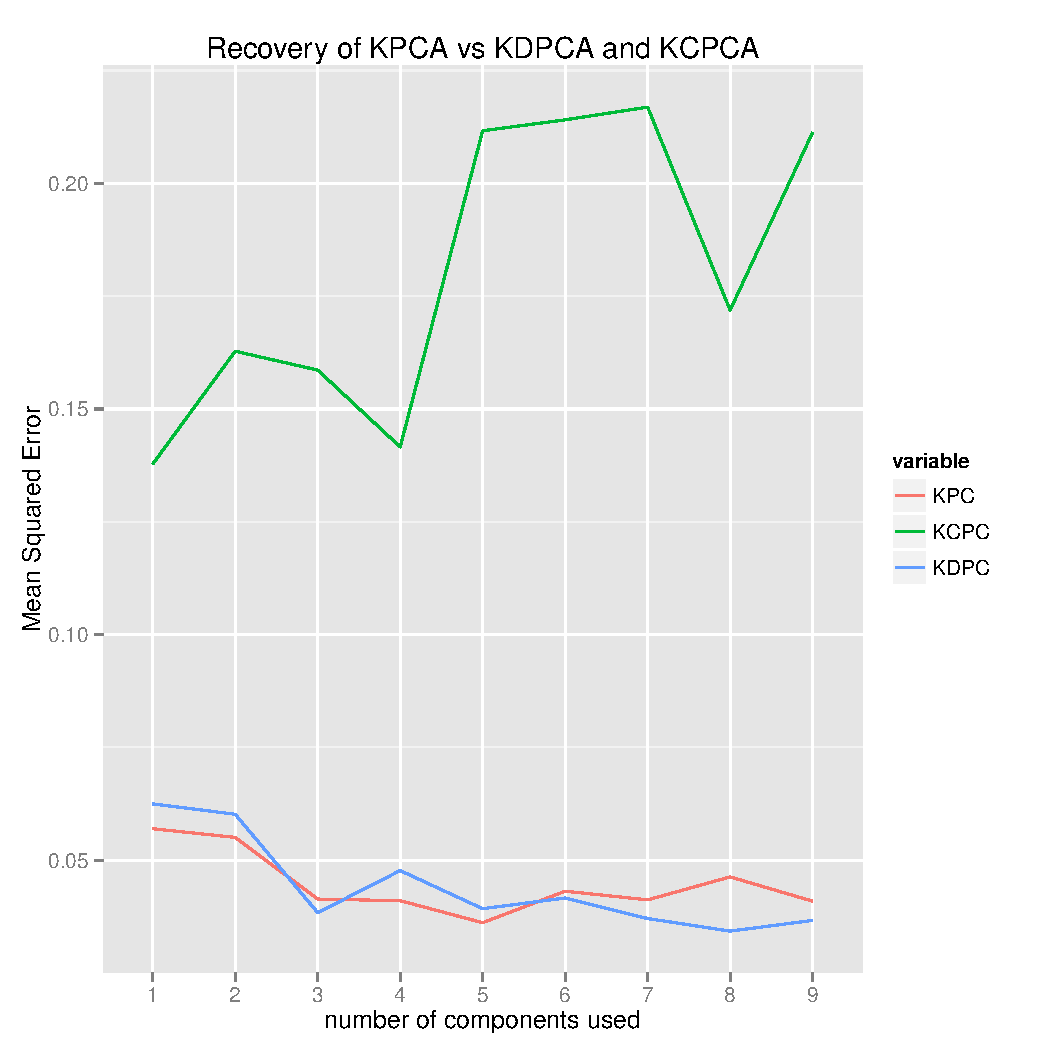
\includegraphics[height = 8cm]{simulation1}
\caption{Mean squared error after recovery of kCPCA, kSPCA and kDPCA}
\label{fig:sim1}
\end{figure*}

\begin{figure*}[htp]
\centering
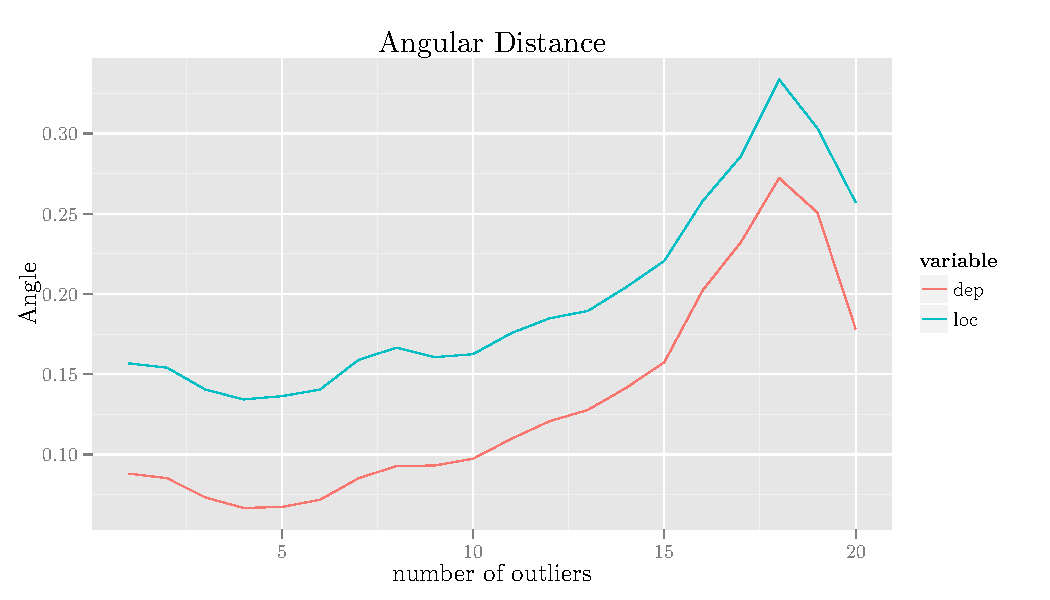
\includegraphics[height=8cm]{simulation2plot}
\caption{Cosine distance measure of the principle components of kCPCA and kDPCA}
\label{fig:sim2}
\end{figure*}

\begin{figure*}[htp]
\captionsetup{justification=centering}
\centering

\subfigure[]{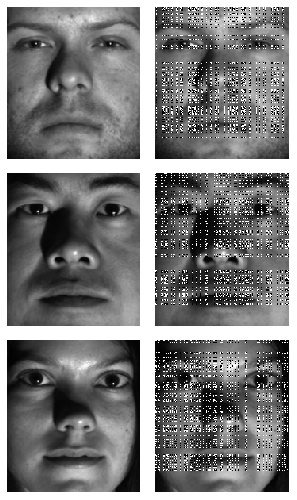
\includegraphics[width=.2\linewidth]{yale1.png}}\qquad
\subfigure[]{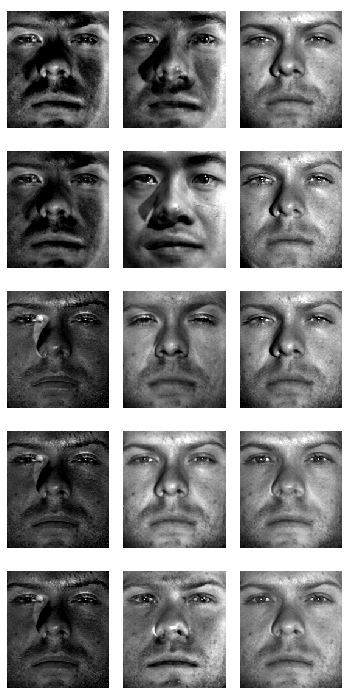
\includegraphics[width=.3\linewidth]{yaleB01recon.png}}\\
\vspace{.5cm}
\subfigure[]{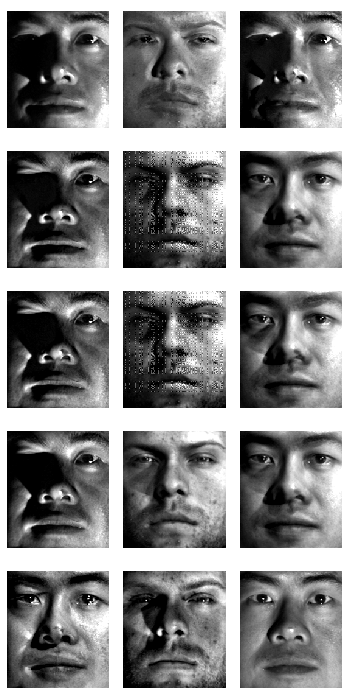
\includegraphics[width=.3\linewidth]{yaleB02recon.png}}\qquad
\subfigure[]{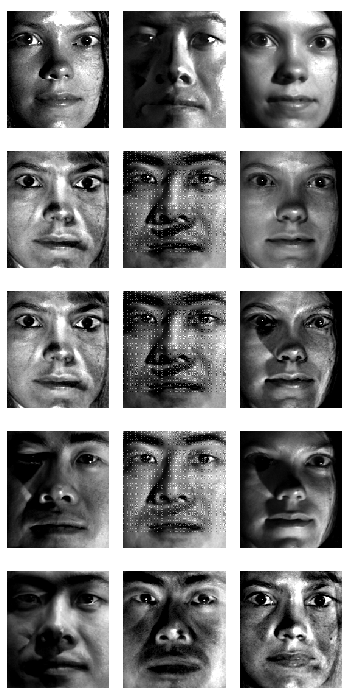
\includegraphics[width=.3\linewidth]{yaleB28recon.png}}
\caption{(a) Original and contaminated images for three persons considered,\\(b), (c) and (d) Reconstructions by kCPCA, kSPCA and kDPCA (in columns) for persons 1, 2 and 3 respectively}
\label{fig:yale1}
\end{figure*}

\end{document}